% Created 2016-11-10 Do 13:17
\documentclass[bigger]{beamer}
\usepackage[utf8]{inputenc}
\usepackage[T1]{fontenc}
\usepackage{fixltx2e}
\usepackage{graphicx}
\usepackage{longtable}
\usepackage{float}
\usepackage{wrapfig}
\usepackage{rotating}
\usepackage[normalem]{ulem}
\usepackage{amsmath}
\usepackage{textcomp}
\usepackage{marvosym}
\usepackage{wasysym}
\usepackage{amssymb}
\usepackage{hyperref}
\usepackage{enumerate}
\usepackage{pdfpages}
\usepackage{multicol}
\usepackage{hyperref}

\tolerance=1000

\author{Matthias Bock}
\date{\textit{[11. November 2016]}}
\title{The Python Imaging Library}
\hypersetup{
  pdfkeywords={PIL Pillow},
  pdfsubject={Praesentation PIL},
  pdfcreator={Bluefish}}
\begin{document}

\maketitle

\frame{
	\frametitle{Was ist PIL ?}
	\begin{itemize}
	\item eine m\"achtige Python-Bibliothek
	\item zur Skript-gesteuerten \textbf{Bildbearbeitung}
	\item geschrieben in Python und C
	\end{itemize}
	}

\frame{
	\frametitle{Was kann PIL ?}
	\begin{center}
		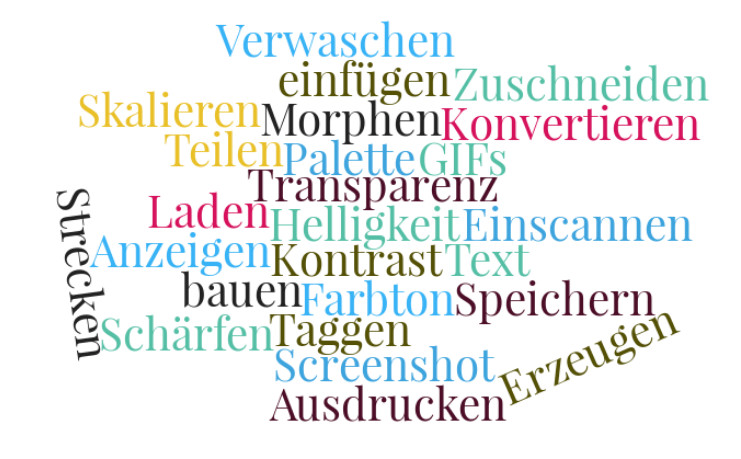
\includegraphics[width=0.95\textwidth]{wordcloud.png}
	\end{center}
	}

\frame{
	\frametitle{PIl ist aufgeteilt in Klassen}
	\begin{center}
		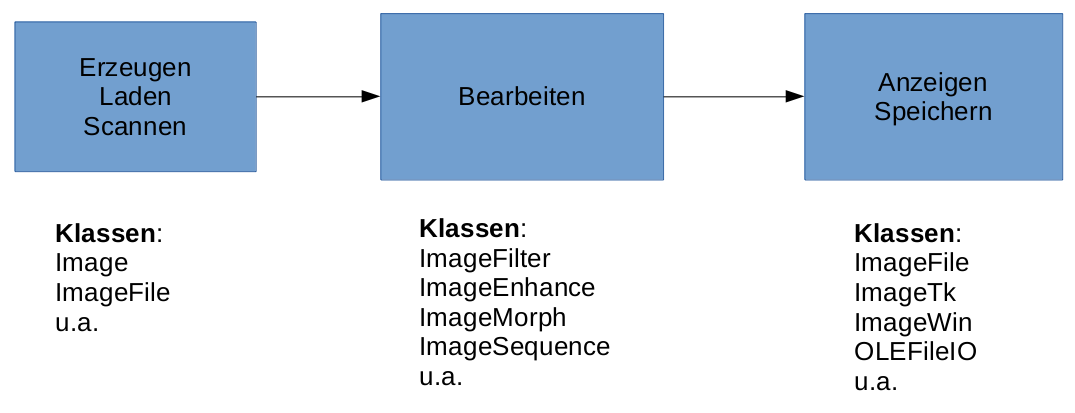
\includegraphics[width=\textwidth]{Flussdiagramm.png}
	\end{center}
}

\frame{
	\frametitle{Beispiel: Pixel-Manipulation}
	\begin{center}
		\fbox{
\includegraphics[width=0.7\textwidth, height=0.4\textheight]{../art.png}}
	\end{center}
	\begin{itemize}
		\item Image.getpixel$\left(\left(x, y\right)\right)$
		\item Image.putpixel$\left(\left(x, y\right), color\right)$
		\item Image.load$\left(\right)$
		\item ImageColor.getrgb$\left("\#rrggbb"\right)$
	\end{itemize}	
}

\frame{
	\frametitle{Beispiel: Bilder zuschneiden}
	\begin{center}
		\fbox{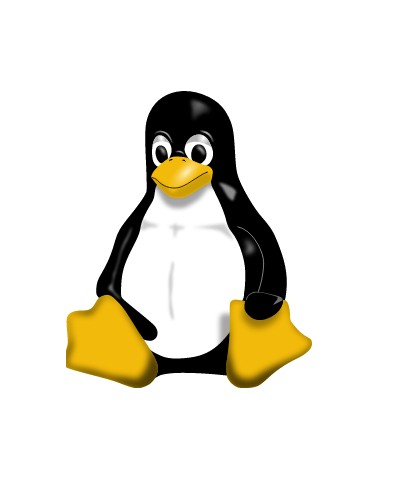
\includegraphics[scale=0.3]{../tux.png}}
		$\Rightarrow$
		\fbox{
\includegraphics[scale=0.3]{../tux-cropped.png}}
	\end{center}
	\begin{itemize}
		\item Image.crop$\left(\right)$
	\end{itemize}
	}

\frame{
	\frametitle{Beispiel: Automatischer Schatten}
	\begin{center}
		\fbox{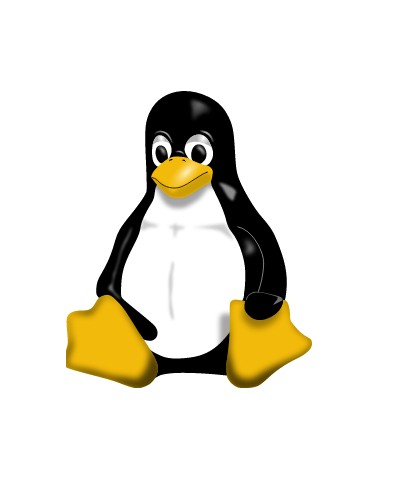
\includegraphics[scale=0.25]{../tux.png}}
		$\Rightarrow$
		\fbox{
\includegraphics[scale=0.25]{../tux+shadow.png}}
	\end{center}
	\begin{itemize}
		\item Image.copy$\left(\right)$
		\item Image.paste$\left(another\_image\right)$
		\item ImageFilter.BLUR
	\end{itemize}
	}

\frame{
\frametitle{Beispiel: Bearbeiten mit Formeln}
\begin{center}
Bild A:
\fbox{
\includegraphics[width=180px]{../beuth-original.png}}

Bild B:
\fbox{
\includegraphics[width=180px]{../beuth-verarbeitet.png}}
\end{center}
	\begin{itemize}
		\item Ist ein Unterschied zu erkennen ?
	\end{itemize}
}

\frame{
\frametitle{Beispiel: Bearbeiten mit Formeln}
\begin{center}
(Bild B - Bild A) * 255:\newline
\fbox{
\includegraphics[width=180px]{../steganographie.png}}
\end{center}
	\begin{itemize}
		\item layers = Image.split$\left(\right)$
		\item new\_layer = ImageMath.eval$\left(expression, layers\right)$
		\item new\_image = Image.merge$\left(mode, \left(new\_layers\right)\right)$
	\end{itemize}
}

\frame{
	\frametitle{Beispiel: Batch-Bearbeitung}
	\begin{center}
		\fbox{
\includegraphics[scale=0.3]{../tux-cropped.png}}
		$\Rightarrow$
		\fbox{\includegraphics[scale=0.18]{../tux-cropped-enhanced.jpg}}
	\end{center}
	\begin{itemize}
		\item os.listdir$\left(path\right)$
		\item Image.resize$\left(new\_size\_tuple\right)$
		\item ImageEnhance.Brightness$\left(\right)$.enhance$\left(magnitude\right)$
		\item ImageEnhance.Contrast$\left(\right)$.enhance$\left(magnitude\right)$
		\item ImageEnhance.Sharpness$\left(\right)$.enhance$\left(factor\right)$
	\end{itemize}
	}

\frame{
	\frametitle{Verf\"ugbarkeit}
	\begin{center}
		\begin{multicols}{2}
			\raggedright
			Debian
			\newline
			Raspbian
			\newline
			Ubuntu
			\newline
			CentOS
			\newline
			RedHat
			\newline
			Fedora
			\newline
			Gentoo
			\newline
			Arch
			\newline
			FreeBSD
			\newline
			MacOSX
			\newline
			Windows 7
			\newline
			Windows 8
		\end{multicols}
	\end{center}
	u.a.
	\newline
	ansonten: aus den Quellen compilieren...
	}

\frame{
\begin{center}
\textbf{Vielen Dank f\"ur Eure Aufmerksamkeit!}
\newline
\newline
\newline
\newline
Fragen?
\end{center}
}

\frame{
	\frametitle{Links und Literatur}
	\begin{itemize}
		\item Homepage (ab 2011): \url{https://python-pillow.org/}
		\item Referenz (ab 2011): \url{http://pillow.readthedocs.io/en/latest/}
		\item Homepage (bis 2011): \url{http://www.pythonware.com/library/pil/handbook/}
		\item Referenz (bis 2011): \url{http://effbot.org/imagingbook/}
		\item Wiki-Buch: \url{https://en.wikibooks.org/wiki/Python\_Imaging\_Library}
	\end{itemize}
	}

\end{document}
